%%%%%%%%%%%%%%%%%%%%%%%%%%%%%%%%%%%%%%%%%%%%%%%%%%%%%%%%%%%%%%%%%%%%%%%%
\chapter{Sistemi ideali di Bose--Einstein}
%%%%%%%%%%%%%%%%%%%%%%%%%%%%%%%%%%%%%%%%%%%%%%%%%%%%%%%%%%%%%%%%%%%%%%%%
\label{cap:bose}

%%%%%%%%%%%%%%%%%%%%%%%%%%%%%%%%%%%%%%%%%%%%%%%%%%%%%%%%%%%%%%%%%%%%%%%%
\section{Equazioni fondamentali per un gas ideale di Bose--Einstein}
%%%%%%%%%%%%%%%%%%%%%%%%%%%%%%%%%%%%%%%%%%%%%%%%%%%%%%%%%%%%%%%%%%%%%%%%

Torniamo alle formule fondamentali per un gas ideale di BE:
%%%%%
\bea
\label{eq:bosefund}
\dfrac{PV}{kT} &=& \ln\calQ = -\sum_\eps\ln\left(1 - \zembe\right) \nonumber\\
%%%%%
N              &=& \sum_\eps \langle n_\eps\rangle = \sum_\eps \dfrac{1}{\zmebe-1}
\eea
%%%%%
Ricordiamo che la fugacità $z$ è collegata al potenziale chimico $\mu$:
%%%%%
\be
z \equiv e^{\mu/kT}
\ee
%%%%%
e che la quantità $\zembe$ deve essere minore di $1$ per qualsiasi valore di $\eps$.

Poiché siamo interessati al limite termodinamico dobbiamo considerare il limite di grandissimi valori di $V$; in questo limite i livelli di energia di singola particella diventano così fitti che sembra lecito, nelle (\ref{eq:bosefund}), sostituire integrali alle somme, a patto di utilizzare la densità degli stati non--relativistica:
%%%%%
\be
a(\eps)\de\eps = \dfrac{2\pi V}{h^3}(2m)^{3/2}\eps^{1/2}\de\eps
\ee
%%%%%
Notiamo tuttavia che il fattore $\eps^{1/2}$ in $a(\eps)$ fa in modo che al livello $\eps=0$ venga dato peso statistico nullo. Mentre questo da un lato sembra inessenziale, visto che in fondo stiamo solo eliminando dall'integrale un insieme di misura nullo, dall'altro è scorretto da un punto di vista di principio. I più curiosi potranno trovare risposta a questo dilemma nell'appendice F del Pathria (terza edizione), nella quale la sommatoria sui livelli di energia è trattata esattamente. La risposta finale, in ogni caso, è la stessa che troveremo seguendo questa strategia semplificata. Per sicurezza riscriviamo le somme separando i termini con $\eps=0$:
%%%%%
\bea
\dfrac{P}{kT} &=& -\dfrac{\ln(1 - z)}{V} - \dfrac{1}{V}\sum_{\eps>0}\ln\left(1 - \zembe\right) \nonumber\\
%%%%%
\dfrac{N}{V}  &=& \dfrac{N_0}{V} + \dfrac{1}{V}\sum_{\eps>0}\dfrac{1}{\zmebe-1}
\eea
%%%%%
in cui $N_0 = z/(1-z)$ rappresenta il numero di bosoni nel livello di energia $\eps=0$. Questo termine ha tutta l'aria di diventare pericoloso quando $z\to 1$. Per il momento notiamo solo che possiamo ricavare $z = N_0/(1+N_0)$ e quindi il primo termine a destra nella prima delle equazioni che precedono può essere scritto come $\ln(1+N_0)/V$. Poiché $N_0$ non può eccedere $N$ otteniamo che questo termine svanisce logaritmicamente nel limite termodinamico; quindi non ce ne occuperemo più.

Adesso alle somme possiamo sostituire gli integrali senza pericolo, estendendo comunque gli integrali da $0$ a $\infty$, perché in ogni caso il termine $\eps=0$ è soppresso dalla densità degli stati. Per la densità numerica, $n = N/V$, otteniamo dunque
%%%%%
\be
\label{eq:nintbose1}
\dfrac{N}{V} = \dfrac{1}{V}\dfrac{z}{1-z} + \dfrac{2\pi(2m)^{3/2}}{h^3}\int_0^\infty 
\dfrac{\eps^{1/2}\de\eps}{\zmebe - 1}
\ee
%%%%%
mentre per la pressione
%%%%%
\be
\label{eq:pintbose1}
\dfrac{P}{kT} = - \dfrac{2\pi(2m)^{3/2}}{h^3}\int_0^\infty
\eps^{1/2}\ln\left(1 - \zembe\right)\de\eps
\ee
%%%%%
Nell'ultima equazione abbiamo omesso il termine che abbiamo scoperto andare logaritmicamente a zero nel limite termodinamico. Con il cambio di variabile $\beta\eps = x$ otteniamo, per la (\ref{eq:nintbose1}),
%%%%%
\be
\label{eq:nintbose2}
\dfrac{N-N_0}{V} = \dfrac{2}{\pi^{1/2}}\bfrac{2\pi mkT}{h^2}^{3/2}\int_0^\infty
\dfrac{x^{1/2}}{\zmex-1}\de x
\ee
%%%%%
Introducendo le funzioni di Bose--Einstein
%%%%%
\be
\label{eq:defgBE1}
\gBE{\nu}(z) \equiv \dfrac{1}{\Gamma(\nu)}\int_0^\infty
\dfrac{x^{\nu-1}}{\zmex-1}\de x
\ee
%%%%%
possiamo finalmente scrivere, riconoscendo nell'eq. (\ref{eq:nintbose2}) la lunghezza d'onda termica $\lambda = h/\sqrt{2\pi mkT}$,
%%%%%
\be
\label{eq:nintbose3}
\dfrac{N-N_0}{V} = \dfrac{\gBE{3/2}(z)}{\lambda^3} 
\ee
%%%%%
Con lo stesso cambio di variabile $x = \beta\eps$ otteniamo, per la (\ref{eq:pintbose1}),
%%%%%
\be
\dfrac{P}{kT} = -\dfrac{4}{3\pi^{1/2}\lambda^3}\int_0^\infty\de(x^{3/2})\ln(1-\zemx)
\ee
%%%%%
che possiamo facilmente integrare per parti, ottenendo
%%%%%
\be
\dfrac{P}{kT} = \dfrac{4}{3\pi^{1/2}\lambda^3}\left\{
\int_0^\infty \dfrac{x^{3/2}}{\zmex-1}\de x - \left[x^{3/2}\ln(1-\zemx)\right]_0^\infty
\right\}
\ee
%%%%%
È facile vedere che l'ultimo termine a destra è nullo in entrambi gli estremi d'integrazione, e ricorrendo ancora alle funzioni di Bose--Einstein possiamo finalmente scrivere
%%%%%
\be
\label{eq:pintbose2}
\dfrac{P}{kT} = \dfrac{\gBE{5/2}(z)}{\lambda^3}
\ee
%%%%%

%%%%%%%%%%%%%%%%%%%%%%%%%%%%%%%%%%%%%%%%%%%%%%%%%%%%%%%%%%%%%%%%%%%%%%%%
\section{Espansione del viriale}
%%%%%%%%%%%%%%%%%%%%%%%%%%%%%%%%%%%%%%%%%%%%%%%%%%%%%%%%%%%%%%%%%%%%%%%%

Prima di qualsiasi altra considerazione cerchiamo di ricavare l'energia interna di un gas di Bose ideale. In linea del tutto generale possiamo scrivere
%%%%%
\bea
\label{eq:defUBE}
U &=& -\bfrac{\partial\ln\calQ}{\partial\beta}_{z,V} =  
kT^2\left[\dparu{T}\bfrac{PV}{kT}\right]_{z,V} \nonumber\\
%%%%%
  &=& kT^2 V \gBE{5/2}(z)\dfrac{\de\lambda^{-3}}{\de T} = 
\dfrac{3}{2}kT\dfrac{V}{\lambda^3}\gBE{5/2}(z)
\eea
%%%%%
Per fare i conti abbiamo usato l'eq. (\ref{eq:pintbose2}) e il fatto che $\lambda\propto T^{-1/2}$. Dal confronto tra la (\ref{eq:defUBE}) e la (\ref{eq:pintbose2}) otteniamo subito un risultato assolutamente generale:
%%%%%
\be
\label{eq:relUPBE}
P = \dfrac{2U}{3V}
\ee
%%%%%

Nei capitoli precedenti abbiamo visto che il limite termodinamico classico comporta che il potenziale chimico tende a $-\infty$ per qualsiasi temperatura, e quindi $z\to 0$. Nel limite di $z$ piccoli possiamo espandere le funzioni di Bose--Einstein in serie di Taylor, ottenendo l'importante risultato:
\be
\label{eq:esp0gBE}
\gBE{\nu}(z) = z + \dfrac{z^2}{2^\nu} + \dfrac{z^3}{3^\nu} + \cdots = \sum_{s=1}^\infty \dfrac{z^s}{s^\nu}
\ee
%%%%%%%%%%%%%%%%%%%%%%%%%%%%%%%%%%%%%%%%%%%%%%%%%%%%%%%%%%%%%%%%%%%%%%%%
\begin{Exercise}[title={Espansione delle funzioni di Bose}, label={ex:bosexp}]
Dimostrare la (\ref{eq:esp0gBE}).

[{\em Suggerimento}\ Utilizzare la definizione di funzione $\Gamma$, eq. (\ref{eq:defGamma}), per il calcolo degli integrali.]$\quad\bullet$ 
\end{Exercise}
%%%%%%%%%%%%%%%%%%%%%%%%%%%%%%%%%%%%%%%%%%%%%%%%%%%%%%%%%%%%%%%%%%%%%%%%
Se ci fermiamo al primo termine dell'espansione otteniamo il limite classico. Infatti in questo limite ($z$ molto piccolo) abbiamo $N_0 \simeq z$ e possiamo quindi trascurarlo rispetto a $N$, che è una quantità estensiva. Possiamo subito scrivere 
\bea
\dfrac{N}{V} &\simeq& \dfrac{z}{\lambda^3} \nonumber\\
\dfrac{P}{kT} &\simeq& \dfrac{z}{\lambda^3}
\eea
Eliminando la $z$, come da prescrizione, otteniamo l'equazione di stato:
\be
PV = NkT
\ee
Notiamo che al primo ordine otteniamo $z = n\lambda^3$; questo risultato sottolinea ancora una volta come il vero parametro d'espansione intorno al caso classico sia $n\lambda^3$.

Se $z$ è piccolo ma non completamente trascurabile, non è una cattiva idea tenere conto del secondo termine dell'espansione in serie delle $\gBE{\nu}(z)$. In questo modo catturiamo i primi effetti puramente quantistici:
\bea
\label{eq:virBE1}
n\lambda^3 = \dfrac{N\lambda^3}{V} &=& z + \dfrac{z^2}{2\sqrt{2}} + \cdots \nonumber\\
\dfrac{P\lambda^3}{kT} &=& z + \dfrac{z^2}{4\sqrt{2}} + \cdots
\eea
Per eliminare $z$ dalle equazioni che precedono dobbiamo invertire la prima serie, ossia ottenere l'espansione di $z$ in termini di $n\lambda^3$, e poi sostituire il risultato nella seconda.
Partendo da $z = n\lambda^3 - z^2/2\sqrt{2}$ possiamo procedere in maniera iterativa, scrivendo:
\bea
z^{(1)} &=& n\lambda^3 \nonumber \\
z^{(2)} &=& n\lambda^3 \left(1 - \dfrac{n\lambda^3}{2\sqrt{2}}\right)
\eea
e qui ci fermiamo perché abbiamo raggiunto il secondo ordine. Sostituendo (con cautela, tenendo conto che dobbiamo rimanere al secondo ordine) nella seconda delle (\ref{eq:virBE1}) otteniamo
\be
\dfrac{P\lambda^3}{kT} = n\lambda^3\left(1 - \dfrac{n\lambda^3}{4\sqrt{2}}\right)
\ee
e in definitiva
\be
\dfrac{PV}{NkT} = 1 - \dfrac{n\lambda^3}{4\sqrt{2}}
\ee
Per un gas ideale classico avremmo ottenuto $PV/NkT = 1$. Vediamo subito che nel caso dei un gas ideale di Bose, almeno in prima approssimazione, riotteniamo un risultato che abbiamo già visto nei capitoli precedenti, ossia che a parità di $N$, $V$ e $T$ la pressione $P$ è {\em inferiore} a quella che si otterrebbe nel caso classico.

Abbiamo appena calcolato il primo termine non banale di quella che si chiama {\em espansione in serie del viriale}. Le serie definite dalle (\ref{eq:virBE1}) possono essere invertite esattamente, e il risultato, una volta eliminata $z$ in favore di $n\lambda^3$, è:
\be
\label{eq:virBEtot}
\dfrac{PV}{NkT} = \sum_{\ell=1}^\infty a_\ell \left( n\lambda^3\right)^{\ell-1}
\ee
I coefficienti del viriale, $a_\ell$, possono essere calcolati termine a termine con la tecnica mostrata sopra. Il primo termine è ovviamente $a_1 = 1$, e abbiamo appena calcolato il primo termine non banale, $a_2 = -1/4\sqrt{2}$.
%%%%%%%%%%%%%%%%%%%%%%%%%%%%%%%%%%%%%%%%%%%%%%%%%%%%%%%%%%%%%%%%%%%%%%%%
\begin{Exercise}[title={Terzo coefficiente}, label={ex:bosevir}]
Ricavare il coefficiente $a_3$ dell'espansione del viriale per un gas ideale di Bose.$\quad\bullet$
\end{Exercise}
%%%%%%%%%%%%%%%%%%%%%%%%%%%%%%%%%%%%%%%%%%%%%%%%%%%%%%%%%%%%%%%%%%%%%%%%
Possiamo ottenere un primo risultato particolare: se ci fermiamo al primo ordine non banale dello sviluppo, utilizzando la (\ref{eq:relUPBE}) otteniamo, per il calore specifico a volume costante,
\be
\dfrac{C_V}{Nk} = \dfrac{1}{Nk}\bfrac{\partial U}{\partial T}_{N,V} =
\dfrac{3}{2}\left[\dparu{T}\bfrac{PV}{Nk}\right]_{N,V}
\ee
Ricordando che $\lambda^3 = cT^{-3/2}$ in cui $c$ non dipende da $T$, troviamo
\be
\dfrac{C_V}{Nk} = \dfrac{3}{2}\dfrac{\de}{\de T}\left(T + a_2ncT^{-1/2}\right)
= \dfrac{3}{2}\left(1-\dfrac{1}{2}a_2 n\lambda^3\right)
\ee
Sappiamo che nel limite classico $C_V/Nk$ deve andare al valore $3/2$, e qui, come prima correzione, abbiamo ottenuto un valore più grande di $3/2$, perché il secondo coefficiente del viriale è negativo; d'altronde sappiamo anche che nel limite $T\to0$ il calore specifico si annulla. Questo significa che da qualche parte il calore specifico deve avere un massimo. Nel seguito vedremo che questo massimo ha il carattere di una cuspide ed è collegato a una transizione di fase molto particolare.

%%%%%%%%%%%%%%%%%%%%%%%%%%%%%%%%%%%%%%%%%%%%%%%%%%%%%%%%%%%%%%%%%%%%%%%%
\section{Transizione di fase di Bose--Einstein}
%%%%%%%%%%%%%%%%%%%%%%%%%%%%%%%%%%%%%%%%%%%%%%%%%%%%%%%%%%%%%%%%%%%%%%%%

Quando $T$ va verso zero e il parametro $n\lambda^3$ cresce, la serie del viriale non ci è più di nessun aiuto. Chiamando $N_e$ il numero di bosoni nei livelli di energia $\eps > 0$, quindi $N_e = N - N_0$, il valore di $z$ deve essere ricavato risolvendo l'equazione implicita
\be
\label{eq:defNeBE}
N_e = \dfrac{V\gBE{3/2}(z)}{\lambda^3}
\ee
Come abbiamo visto in precedenza, se $z \ll 1$ allora $N_0$ è trascurabile rispetto a $N$ e quindi $N_e \simeq N$. Le cose cambiano drasticamente quando $z\simeq 1$ (ricordiamo che $0 \le z \le 1$). Quando $z$ si avvicina a $1$ dobbiamo capire cosa succede alla funzione $\gBE{3/2}(z)$. Dalla sua espansione in serie vediamo subito che $\gBE{3/2}(z)$ cresce monotonicamente con $z$ e raggiunge il suo massimo per $z=1$:
\be
\gBE{3/2}(1) = 1 + \dfrac{1}{2^{3/2}} + \dfrac{1}{3^{3/2}} + \cdots
= \sum_{s=1}^\infty \dfrac{1}{s^{3/2}} \equiv \zeta(3/2)
\ee
in cui $\zeta(x)$ è la funzione $\zeta$ di Riemann, e sappiamo che $\zeta(3/2) = 2.612\dots$

Se ora riconsideriamo l'eq. (\ref{eq:defNeBE}) troviamo una sorpresa: per $V$ e $T$ fissati il valore di $N_e$ è limitato:
\be
\label{eq:limNe}
N_e \le \dfrac{V}{\lambda^3}\zeta(3/2)
\ee
Ora, finché $N$ è minore di questo valore limite va tutto bene: i bosoni sono distribuiti sugli stati $\eps > 0$, a tutti gli effetti pratici $N \simeq N_e$ e il valore di $z$ è determinato dalla soluzione dell'eq. (\ref{eq:defNeBE}).

Ma il fisico quadratico medio, si sa, è perverso: cosa succederà mai, si chiede il mefistofelico personaggio, se a $T$ e $V$ fissati continuo a inserire bosoni nel sistema {\em dopo} che il limite critico (\ref{eq:limNe}) è stato raggiunto? È evidente che questi {\em nuovi} bosoni non possono essere accomodati nei livelli $\eps>0$, visto che il limite critico è stato raggiunto e superato. A queste particelle non resta altro da fare se non precipitare il prima che sia possibile nello stato $\eps=0$, andando così a incrementare il valore di $N_0$. Va notato che nulla vieta a $N_0$ di aumentare in maniera indefinita. A questo punto $z$ non può più essere calcolata tramite la (\ref{eq:defNeBE}); dobbiamo invece usare la formula
\be
z = \dfrac{N_0}{N_0+1}\simeq 1 - \dfrac{1}{N_0}
\ee
che ci restituisce un valore molto prossimo a $1$, visto che $N_0$ può crescere senza limiti.

Il fenomeno per cui i bosoni si accumulano sul livello $\eps=0$ è conosciuto come {\em condensazione di Bose--Einstein}. È molto simile a una transizione di fase, e anzi, di fatto la è, a patto che non si dimentichi che è una transizione nello spazio dei momenti (o delle energie) e non nello spazio delle coordinate. Inoltre la sua origine è puramente quantistica, visto che abbiamo completamente trascurato gli effetti dovuti alle interazioni tra particelle.

Finora abbiamo tenuto $V$ e $T$ costanti e variato $N$, ottenendo la condizione perché si verifichi la condensazione di Bose--Einstein:
\be
\label{eq:disdens}
\dfrac{N}{V} > T^{3/2}\bfrac{2\pi mk}{h^2}^{3/2}\zeta(3/2)
\ee
Possiamo ora chiederci cosa succede se partiamo da una situazione in cui il sistema, in equilibrio a una certa temperatura $T$, non è condensato, e quindi con una densità minore della densità critica definita dalla (\ref{eq:disdens}). Possiamo pensare di abbassare la temperatura, mantendendo la densità costante; a un certo punto, arrivati a una temperatura critica $T_c$, la diseguaglianza (\ref{eq:disdens}) verrà comunque soddisfatta, anche tenendo costante il rapporto $N/V$. Otteniamo così una temperatura critica
\be
\label{eq:TCBE}
T_c = \dfrac{h^2}{2\pi mk}\left[\dfrac{N}{V\zeta(3/2)}\right]^{2/3}
\ee
Per $T > T_c$ il numero di particelle nel livello $\eps = 0$, cioè $z/(1-z)$, è $O(1)$, cioè completamente trascurabile rispetto a $N$.

La situazione cambia drasticamente per $T < T_c$; in questo caso il sistema può essere visto come una mistura di due fasi:
\begin{enumerate}
\item una {\em fase normale}, composta da $N_e$ particelle distribuite sui livelli $\eps > 0$, e la frazione di particelle $N_e/N$ è pari a $(T/T_c)^{3/2}$
\item una {\em fase condensata}, composta da $N_0 = N-N_e$ particelle accumulate nel livello $\eps = 0$.
\end{enumerate}
Il risultato $N_e/N = (T/T_c)^{3/2}$ può essere ricavato in questo modo. Esattamente a temperatura critica il valore di $N_0$ è ancora trascurabile rispetto a $N$, quindi la (\ref{eq:TCBE}) ci dice che $N = cT_c^{3/2}$ in cui $c$ è una costante. Appena scendiamo a una temperatura $T$ sotto temperatura critica, una frazione finita di particelle deve condensare nel livello $\eps=0$, e la stessa equazione ci dice che il numero di particelle che rimangono sui livelli $\eps>0$ è: $N_e = cT^{3/2}$. Dal rapporto otteniamo il risultato esposto. In figura (\ref{fig:n0sun}) sono mostrati graficamente i comportamenti di $N_0/N$ e di $N_e/N$ in funzione di $T/T_c$.
%%%%%%%%%%%%%%%%%%%%%%%%%%%%%%%%%%%%%%%%%%%%%%%%%%%%%%%%%%%%%%%%%%%%%%
\begin{figure}[!ht]
	\centering
	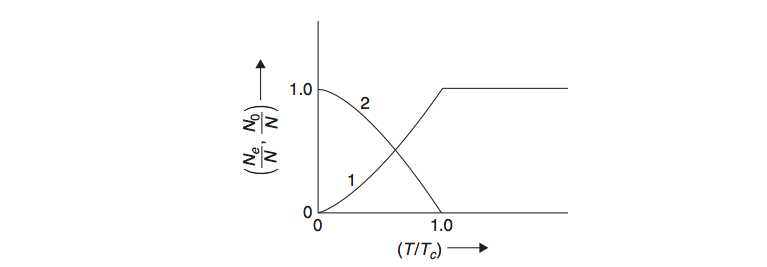
\includegraphics[width=1.0\textwidth]{Bose-N0suN.png}
	\caption{Frazione del numero di particelle nella fase normale e nella fase condensata in funzione di $T/T_c$.}
	\label{fig:n0sun}
\end{figure}
%%%%%%%%%%%%%%%%%%%%%%%%%%%%%%%%%%%%%%%%%%%%%%%%%%%%%%%%%%%%%%%%%%%%%%

È interessante anche capire la variazione di $z$ al variare di $T$, ma è più semplice considerare $z$ come funzione di $v/\lambda^3$. Ricordiamo che $v$ è il volume specifico, ossia l'inverso della densità $n$: $v = V/N$. Di conseguenza $v/\lambda^3$ è proporzionale a $T^{3/2}$. Per $T < T_c$ abbiamo visto che vale $z \simeq 1 - 1/N_0$, e poiché nel limite termodinamico $N_0$ diverge abbiamo $z \simeq 1$. Sempre dalla (\ref{eq:TCBE}) abbiamo che il valore critico di $v/\lambda^3$, cioè il valore corrispondente a $T_c$, è pari a $1/\zeta(3/2)$, che vale circa $(2.612)^{-1}$.
Per $v/\lambda^3 > (2.612)^{-1}$ il valore di $z$ è determinato implicitamente dalla relazione
\be
\gBE{3/2}(z) = \lambda^3/v < 2.612
\ee
Per valori molto grandi di $v/\lambda^3$, e cioè per valori molto piccoli di $n\lambda^3$, ritroviamo la situazione classica, ossia $z\simeq (v/\lambda^3)^{-1}$. La situazione è riassunta in figura (\ref{fig:zvsT}).
%%%%%%%%%%%%%%%%%%%%%%%%%%%%%%%%%%%%%%%%%%%%%%%%%%%%%%%%%%%%%%%%%%%%%%
\begin{figure}[!ht]
	\centering
	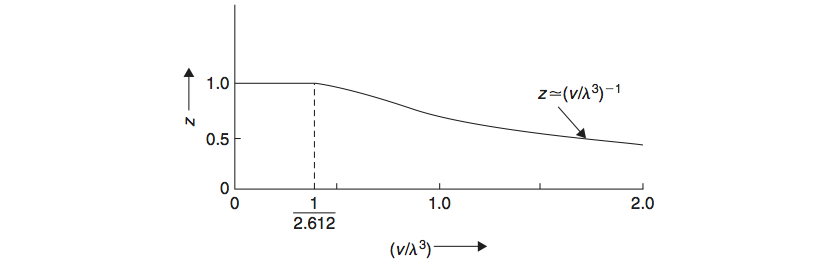
\includegraphics[width=1.0\textwidth]{Bose-zvsT.png}
	\caption{Fugacità di un gas ideale di Bose in funzione di $v/\lambda^3$.}
	\label{fig:zvsT}
\end{figure}
%%%%%%%%%%%%%%%%%%%%%%%%%%%%%%%%%%%%%%%%%%%%%%%%%%%%%%%%%%%%%%%%%%%%%%

%%%%%%%%%%%%%%%%%%%%%%%%%%%%%%%%%%%%%%%%%%%%%%%%%%%%%%%%%%%%%%%%%%%%%%
\section{Termodinamica del gas ideale di Bose}
%%%%%%%%%%%%%%%%%%%%%%%%%%%%%%%%%%%%%%%%%%%%%%%%%%%%%%%%%%%%%%%%%%%%%%

In questa sezione esamineremo le principali caratteristiche termodinamiche di un gas ideale di Bose.

%%%%%%%%%%%%%%%%%%%%%%%%%%%%%%%%%%%%%%%%%%%%%%%%%%%%%%%%%%%%%%%%%%%%%%
\subsection{La pressione}
%%%%%%%%%%%%%%%%%%%%%%%%%%%%%%%%%%%%%%%%%%%%%%%%%%%%%%%%%%%%%%%%%%%%%%

Esaminiamo il diagramma $(P,T)$, cioè la variazione di $P$ in funzione della temperatura $T$ tenendo fissata la densità $n = N/V$ (oppure $v = 1/n$) a un valore costante. Per $T \le T_c$ la pressione è data dall'eq.(\ref{eq:pintbose2}) con $z=1$. Otteniamo quindi
\be
\label{eq:pundertc}
P(T) = \dfrac{kT}{\lambda^3}\zeta(5/2)\quad\quad T \le T_c
\ee
in cui notiamo che la pressione è proporzionale a $T^{5/2}$ ed è indipendente da $V$; ciò significa che in queste condizioni il gas è {\em infinitamente comprimibile}.

Esattamente a temperatura critica, utilizziamo la (\ref{eq:nintbose3}) per scrivere
\be
\dfrac{1}{\lambda^3_c} = \dfrac{N}{V}\dfrac{1}{\zeta(3/2)}
\ee
in cui $\lambda^3_c$ è il valore di $\lambda^3$ per $T=T_c$. Sostituendo la precedente nella (\ref{eq:pundertc}) otteniamo, per la pressione a $T=T_c$:
\be
\label{eq:pattc}
P(T_c) = \dfrac{\zeta(5/2)}{\zeta(3/2)}NkT_c/V
\ee
Il rapporto $\zeta(5/2)/\zeta(3/2)$ vale circa $0.5134$, e dunque vediamo che a temperatura critica la pressione di un gas ideale di Bose è circa la metà del valore che otterremmo per un gas ideale classico.

Per $T > T_c$ il valore della pressione è dato da
\be
\label{eq:povertc}
P(T) = \dfrac{NkT}{V}\dfrac{\gBE{5/2}(z)}{\gBE{3/2}(z)}
\ee
e per eliminare $z$ allo scopo di ottenere l'equazione di stato dobbiamo risolvere la relazione implicita
\be
\gBE{3/2}(z) = n\lambda^3
\ee
A meno di non essere vicini al limite classico, in cui possiamo utilizzare l'espansione del viriale e $P$ tende asintoticamente al valore $NkT/V$, non esiste un modo semplice per esprimere la pressione e occorre adattarsi a una soluzione numerica. La situazione è riassunta in figura
(\ref{fig:PvsT}).
%%%%%%%%%%%%%%%%%%%%%%%%%%%%%%%%%%%%%%%%%%%%%%%%%%%%%%%%%%%%%%%%%%%%%%
\begin{figure}[!ht]
	\centering
	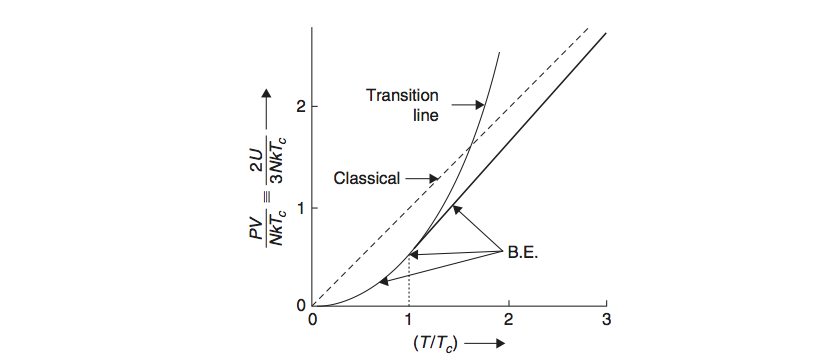
\includegraphics[width=1.0\textwidth]{Bose-PvsT.png}
	\caption{Pressione di un gas ideale di Bose in funzione di $T/T_c$.}
	\label{fig:PvsT}
\end{figure}
%%%%%%%%%%%%%%%%%%%%%%%%%%%%%%%%%%%%%%%%%%%%%%%%%%%%%%%%%%%%%%%%%%%%%%

%%%%%%%%%%%%%%%%%%%%%%%%%%%%%%%%%%%%%%%%%%%%%%%%%%%%%%%%%%%%%%%%%%%%%%
\subsection{Il calore specifico}
%%%%%%%%%%%%%%%%%%%%%%%%%%%%%%%%%%%%%%%%%%%%%%%%%%%%%%%%%%%%%%%%%%%%%%

Per calcolare il calore specifico a volume costante sotto la temperatura critica possiamo sfruttare la relazione che lega l'energia interna alla pressione e al volume:
\be
U = \dfrac{3}{2}PV
\ee
e quindi fare uso del'eq. (\ref{eq:pundertc}). Tenendo conto che $C_V = (\partial U/\partial T)_{N,V}$, possiamo scrivere
\be
\dfrac{C_V}{Nk}  = \dfrac{3V}{2N}\,\zeta(5/2)\dfrac{\de}{\de T}\bfrac{T}{\lambda^3}
= \dfrac{15}{4}\,\zeta(5/2)\dfrac{v}{\lambda^3}\quad\quad T < T_c
\ee
Vediamo quindi che quando $T$ va a zero, $C_V\to 0$ come $T^{3/2}$. 

Esattamente a $T = T_c$ abbiamo
\be
\dfrac{C_V(T_c)}{Nk} = \dfrac{15\,\zeta(5/2)}{4\,\zeta(3/2)} \simeq 1.925
\ee
che è considerevolmente più grande del valore classico pari a $3/2$.

Per $T>T_c$, ma lontani dal limite classico, tutto quel che possiamo ottenere è come al solito una relazione implicita. Utilizzando le espressioni generali per $P$ e per $N$ e la relazione che lega $U$ a $P$ otteniamo facilmente
\be
\label{eq:cvgeneric}
\dfrac{C_V}{Nk} = \dfrac{3}{2}\dfrac{\partial}{\partial T}\left(T\,\dfrac{\gBE{5/2}(z)}{\gBE{3/2}(z)}  \right)_{N,V}
\ee
il problema della quale consiste nel capire come calcolare $(\partial z/\partial T)_{N,V}$. Possiamo infatti scrivere
\be
\dfrac{C_V}{Nk} = \dfrac{3}{2}\left[\dfrac{\gBE{5/2}(z)}{\gBE{3/2}(z)}
+ T\dpard{z}{T}{N}{V}\dfrac{\partial}{\partial z}\bfrac{\gBE{5/2}(z)}{\gBE{3/2}(z)}\right]
\ee
Occupiamoci prima di tutto dell'ultima derivata. Scrivendo le funzione di Bose $\gBE{\nu}(z)$ in serie di potenze,
\be
\gBE{\nu}(z) = z + \dfrac{z^2}{2^\nu} + \dfrac{z^3}{3^\nu} + \cdots
\ee
ci accorgiamo subito che valgono le relazioni di ricorsione:
\be
\label{eq:grec}
z\dpar{\gBE{\nu}(z)}{z} = z + \dfrac{z^2}{2^{\nu-1}} + \dfrac{z^3}{3^{\nu-1}} + \cdots = \gBE{\nu-1}(z)
\ee
per cui otteniamo facilmente
\be
\label{eq:derz}
\dfrac{\partial}{\partial z}\bfrac{\gBE{5/2}(z)}{\gBE{3/2}(z)} = 
\dfrac{1}{z}\left(1 - \dfrac{\gBE{5/2}(z)\gBE{1/2}(z)}{\gBE{3/2}^2(z)} \right)
\ee
Poi notiamo che poiché $\gBE{3/2}(z) \propto T^{-3/2}$ allora
\be
\left[\dparu{T}\gBE{3/2}(z)\right]_{N,V} = -\dfrac{3}{2T}\gBE{3/2}(z)
\ee
ma avremmo ben potuto scrivere
\be
\left[\dparu{T}\gBE{3/2}(z)\right]_{N,V} = \dpard{z}{T}{N}{V}\dfrac{\partial\gBE{3/2}(z)}{\partial z} = \dpard{z}{T}{N}{V} \dfrac{1}{z}\,\gBE{1/2}(z)
\ee
in cui nell'ultimo passaggio abbiamo usato la relazione di ricorsione (\ref{eq:grec}). Otteniamo quindi
\be
\dpard{z}{T}{N}{V} = -\dfrac{3z}{2T}\dfrac{\gBE{3/2}(z)}{\gBE{1/2}(z)}
\ee
Utilizzando tutti i risultati parziali possiamo finalmente scrivere
\be
\label{eq:cvbose}
\dfrac{C_V}{Nk} = \dfrac{15\,\gBE{5/2}(z)}{4\,\gBE{3/2}(z)} - \dfrac{9\,\gBE{3/2}(z)}{4\,\gBE{1/2}(z)}
\ee
nella quale come al solito a $z$ come funzione di $T$ occorre sostituire il valore ricavato dall'equazione implitica $n\lambda^3 = \gBE{3/2}(z)$. Nel limite $z\to 1$ il secondo termine si annulla a causa della divergenza di $\gBE{1/2}(z)$ e recuperiamo il valore che avevamo calcolato per $T = T_c$; lo stesso limite che otteniamo arrivando a $T_c$ dal basso. Questo significa che il calore specifico è continuo alla transizione. La sua derivata, tuttavia, presenta una discontinuità.
%%%%%%%%%%%%%%%%%%%%%%%%%%%%%%%%%%%%%%%%%%%%%%%%%%%%%%%%%%%%%%%%%%%%%%
\begin{Exercise}
Dimostrare che per un gas di Bose ideale vale la relazione:
\be
\bfrac{\partial C_V}{\partial T}_{T\to T_c^-} -
\bfrac{\partial C_V}{\partial T}_{T\to T_c^+} =
\dfrac{27\,Nk}{16\,\pi T_c}\zeta^2(3/2)\quad\bullet
\ee
\end{Exercise}
%%%%%%%%%%%%%%%%%%%%%%%%%%%%%%%%%%%%%%%%%%%%%%%%%%%%%%%%%%%%%%%%%%%%%%
\noindent
Per $T > T_c$ il calore specifico decresce verso il suo valore limite classico:
\be
\bfrac{C_V}{Nk}_{z\to0} = \dfrac{15}{4} - \dfrac{9}{4} = \dfrac{3}{2}
\ee

%%%%%%%%%%%%%%%%%%%%%%%%%%%%%%%%%%%%%%%%%%%%%%%%%%%%%%%%%%%%%%%%%%%%%%
\subsection{Isoterme e adiabatiche}
%%%%%%%%%%%%%%%%%%%%%%%%%%%%%%%%%%%%%%%%%%%%%%%%%%%%%%%%%%%%%%%%%%%%%%

Consideriamo la variazione della pressione al variare del volume, tenendo la temperatura fissata. In questo caso otterremo la transizione per un determinato valore critico del volume, o meglio del volume specifico:
\be
v_c = \lambda^3/\zeta(3/2)
\ee
Notiamo che $v_c\propto T^{-3/2}$. Per $v < v_c$ la pressione non dipende dal volume e si riduce all'espressione (\ref{eq:pundertc}). Abbiamo quindi, ricordando che $P_0 \propto T$, 
\be
P_0v_c^{5/3} = \textrm{costante}
\ee
La regione a sinistra di questa linea, nel piano $(P,V)$, appartiene alla fase mista. La linea stessa è la linea di transizione, mentre a destra abbiamo solo la fase normale. La situazione è riassunta in figura (\ref{fig:bose-isoterme}).
%%%%%%%%%%%%%%%%%%%%%%%%%%%%%%%%%%%%%%%%%%%%%%%%%%%%%%%%%%%%%%%%%%%%%%%%
\begin{figure}[!ht]
	\centering
	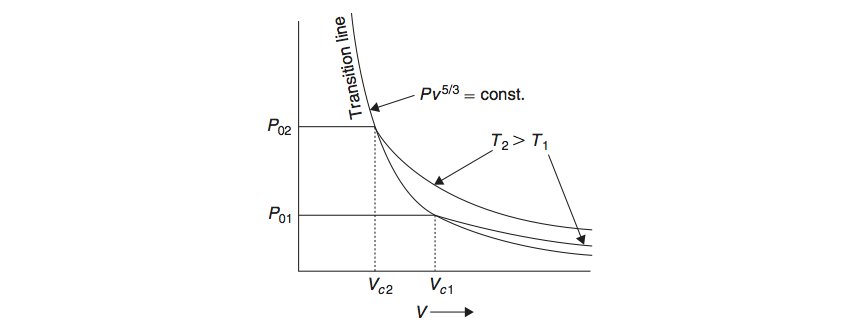
\includegraphics[width=1.0\textwidth]{Bose-isoterme.png}
	\caption{Isoterme di un gas ideale di Bose.}
	\label{fig:bose-isoterme}
\end{figure}
%%%%%%%%%%%%%%%%%%%%%%%%%%%%%%%%%%%%%%%%%%%%%%%%%%%%%%%%%%%%%%%%%%%%%%%%

Per poter studiare le adiabatiche dobbiamo trovare una formula per l'entropia del sistema: utilizzando l'espressione termodinamica
\be
G = U - TS + PV = N\mu
\ee
possiamo scrivere
\be
\dfrac{S}{Nk} = \dfrac{U + PV}{NkT} - \dfrac{\mu}{kT}
\ee
Inseriamo in questa equazione le relazioni ricavate in precedenza per $U$ e $P$, ottenendo:
\bea
\dfrac{S}{Nk} &=& \dfrac{5\,\gBE{5/2}(z)}{2\,\gBE{3/2}(z)} - \ln z\quad\quad T > T_c \nonumber\\
\dfrac{S}{Nk} &=& \dfrac{5}{2}\dfrac{v}{\lambda^3}\,\zeta(5/2)\quad\quad\quad\;\; T \le T_c
\eea
In un processo adiabatico sia $S$ sia $N$ devono rimanere costanti. La prima delle relazioni precedenti implica che sia $z$ sia $v/\lambda^3$ devono rimanere costanti per $T > T_c$. Lo stesso è vero per $T \le T_c$. Per un processo adiabatico otteniamo quindi
\bea
vT^{3/2}  &=& \textrm{costante} \nonumber\\
P/T^{5/2} &=& \textrm{costante}
\eea
ed eliminando $T$ otteniamo l'equazione per un'adiabatica:
\be
Pv^{5/3} = \textrm{costante}
\ee
Notiamo che questo risultato, che vale per ogni temperatura, è identico a quello classico, ma mentre nel caso classico l'esponente $5/3$ è il rapporto $C_P/C_V$ nel caso di Bose questo non è vero. Si può infatti dimostrare che $C_P/C_V > 5/3$ e tende al valore classico solo nel limite $n\lambda^3 \to 0$.

Infine notiamo che per $T < T_c$ possiamo scrivere
\be
S = kN_e\dfrac{5\,\zeta(5/2)}{2\,\zeta(3/2)} \propto N_e
\ee
il che equivale a dire che le particelle nel livello $\eps = 0$ non contribuiscono all'entropia.


%%%%%%%%%%%%%%%%%%%%%%%%%%%%%%%%%%%%%%%%%%%%%%%%%%%%%%%%%%%%%%%%%%%%%%%%
\section{La radiazione di corpo nero}
%%%%%%%%%%%%%%%%%%%%%%%%%%%%%%%%%%%%%%%%%%%%%%%%%%%%%%%%%%%%%%%%%%%%%%%%

La storia del corpo nero inizia intorno al 1860 quando Kirchhoff definisce che
cosa si intende per corpo nero e formula alcune leggi generali sulle sue proprietà. Kirchhoff, basandosi su dati sperimentali, arrivò a enunciare questa legge:
\begin{quote}
Per una data temperatura $T$ e una data frequenza $\nu$ della radiazione elettromagnetica, il rapporto tra potere emissivo e quello d'assorbimento è lo stesso per tutti i corpi.
\end{quote}
In formule possiamo scrivere
\be
\label{eq:funibb}
\dfrac{e(\nu,T)}{a(\nu,T)} = f(\nu,T)
\ee
in cui $f(\nu,T)$ è una funzione universale. Kirchhoff immaginò allora un oggetto il cui potere d'assorbimento fosse pari a $1$, per ogni frequenza e ogni temperatura, e chiamò quest'oggetto {\em corpo nero}. Dalla definizione (\ref{eq:funibb}) è chiaro che la funzione universale $f(\nu,T)$ coincide con la funzione $e_{\text{cn}}(\nu,T)$ d'emissione del corpo nero.

Fu lo stesso Kirchhoff a suggerire un'implementazione pratica dell'oggetto ideale {\em corpo nero}. Immaginò una cavità di volume $V$ tenuta a una temperatura costante $T$: la radiazione all'interno della cavità arriverà, prima o poi, all'equilibrio termico con le pareti del contenitore. Se ora si pratica un piccolo foro in una delle pareti del contenitore, le dimensioni del quale non compromettano l'equilibrio tra radiazione e pareti, la radiazione uscente dal foro avrà tutte le caratteristiche di una radiazione di corpo nero. In questo caso, è bene stare attenti a non confondersi, il corpo nero è rappresentato dal {\em foro}, non dall'interno del contenitore. Infatti le dimensioni del contenitore sono tali che qualsiasi tipo di radiazione entrante nel foro stesso sarà presto assorbita dalle pareti del contenitore, senza poterne riuscire (se non sotto forma di radiazione all'equilibrio termico a temperatura $T$, appunto). Il foro dunque assorbe tutta la radiazione incidente, ed emette secondo la funzione universale di corpo nero.

%%%%%%%%%%%%%%%%%%%%%%%%%%%%%%%%%%%%%%%%%%%%%%%%%%%%%%%%%%%%%%%%%%%%%%%%
\subsection{La teoria di Planck}
%%%%%%%%%%%%%%%%%%%%%%%%%%%%%%%%%%%%%%%%%%%%%%%%%%%%%%%%%%%%%%%%%%%%%%%%
Nel 1900 Planck, nel tentativo di trovare una formula che descrivesse nella maniera corretta l'enorme mole di dati sperimentali che si erano accumulati negli anni precedenti sulla radiazione di corpo nero, ipotizzò che le cariche elettriche presenti sulle pareti della cavità si muovessero come oscillatori armonici, ma con energie quantizzate: $\eps_n = n\hbar\omega$, con $n = 0,\,1,\,2,\,\ldots$, $\omega$ la frequenza (angolare) dell'oscillatore e $\hbar$ una ``costante di natura'' da determinare tramite il confronto con i dati sperimentali. Si noti l'esclusione dell'energia di punto zero, $\hbar\omega/2$, che contribuirebbe all'energia totale del sistema, nel limite termodinamico, come una costante infinita. Ma l'energia è definita a meno di una costante additiva arbitraria, e possiamo tranquillamente trascurare questo termine. Escludendo dunque l'energia di punto zero, utilizzando l'ensemble canonico e, si noti bene, la statistica di MB, l'energia media del singolo oscillatore può essere scritta come 
\be
\label{eq:ensingmod}
\langle \eps \rangle = \dfrac{\hbar\omega}{e^{\hbar\omega/kT} - 1}
\ee
All'equilibrio termico, le onde elettromagnetiche nella cavità avranno le stesse frequenze degli oscillatori armonici. La formula di Rayleigh
\be
\label{eq:rayl}
g(\omega)\de{\omega} = \dfrac{\omega^2}{\pi^2 c^3}\de{\omega}
\ee
rappresenta il numero di modi normali di vibrazione per unità di volume all'interno della cavità, nell'intervallo di frequenze $(\omega,\;\omega+\de{\omega})$. Nel ricavare la formula (\ref{eq:rayl}), in cui $c$ è la velocità della luce, Rayleigh tenne conto del fatto che le onde elettromagnetiche sono solo trasversali e hanno quindi un fattore $2$ di degenerazione.

Se dunque la (\ref{eq:ensingmod}) rappresenta l'energia del singolo modo normale di vibrazione di frequenza $\omega$, basta moltiplicare per la densità degli stati (\ref{eq:rayl}) per ottenere la densità di energia $u(\omega)\de{\omega}$ associata all'intervallo di frequenze
$(\omega,\;\omega+\de{\omega})$:
\be
\label{eq:bbplanck}
u(\omega)\de{\omega} = \dfrac{1}{\pi^2 c^3}\dfrac{\hbar\omega^3}{e^{\hbar\omega/kT} - 1}
\de{\omega}
\ee
che è esattamente la formula di Planck per la distribuzione della densità di energia della radiazione all'interno della cavità. Integrando su tutte le frequenze $\omega$ si ottiene la densità di energia totale.

%%%%%%%%%%%%%%%%%%%%%%%%%%%%%%%%%%%%%%%%%%%%%%%%%%%%%%%%%%%%%%%%%%%%%%%%
\subsection{Il punto di vista di Bose}
%%%%%%%%%%%%%%%%%%%%%%%%%%%%%%%%%%%%%%%%%%%%%%%%%%%%%%%%%%%%%%%%%%%%%%%%
Nel 1924 l'idea che il campo elettromagnetico dovesse essere quantizzato e che esistessero {\em particelle di luce} chiamate fotoni, i quanti del campo, era ormai largamente condivisa; se non altro dai fisici. Un fino ad allora oscuro ricercatore indiano, Bose, non riusciva a farsi pubblicare un articolo in cui derivava la legge di Planck a partire dal concetto di fotone, sulla base di un nuovo tipo di statistica, diversa da quella di Boltzmann. Invece di rassegnarsi all'oblio e sicuro dei suoi risultati, spedì l'articolo ad Einstein, il quale lo trovò così interessante da farlo pubblicare immediatamente. Non solo: in pochi mesi elaborò i risultati di Bose ed estese la nuova statistica a tutte le particelle che ora si chiamano bosoni.

Il lavoro di Bose e Einstein può essere rapidamente riassunto in questo modo. La famosa cavità di cui sopra è piena di particelle di massa nulla e spin pari a $1$: i fotoni. La trasversalità delle onde elettromagnetiche fa sì però che ogni fotone abbia solo $2$ possibili polarizzazioni, e non $3$. Questo gas di particelle ultrarelativistiche è all'equilibrio termico a temperatura $T$, e un singolo fotone di frequenza $\omega$ ha energia pari a $\hbar\omega$. Ci domandiamo quale sia la densità degli stati, in funzione dell'energia, per un gas ultrarelativistico. Il conto è presto fatto, perché possiamo scrivere $\eps = pc$ e usare la densità degli stati in funzione del momento, che abbiamo già calcolato:
\be
g(p)\de{p} = \dfrac{4\pi V}{h^3} p^2\de{p} = \dfrac{V}{2\pi^2\hbar^3} p^2\de{p}
\ee
Passando alle energie, possiamo scrivere
\be
g(\eps)\de{\eps} = \dfrac{V}{2\pi^2\hbar^3 c^3} \eps^2\de{\eps}
\ee
e sapendo che $\eps = \hbar\omega$ abbiamo
\be
g(\omega)\de{\omega} = \dfrac{V}{2\pi^2\hbar^3 c^3} \hbar^3\omega^2\de{\omega}
\ee
Il conto non è ancora completo, perché per ogni fotone abbiamo due possibili stati di polarizzazione, quindi dobbiamo moltiplicare il risultato per un fattore $2$, e se vogliamo ottenere la densità degli stati {\em per unità di volume} dobbiamo ancora dividere per un fattore $V$. Abbiamo dunque
\be
\label{eq:gomega}
g(\omega)\de{\omega} = \dfrac{\omega^2}{\pi^2 c^3}\de{\omega}
\ee
che senza troppe sorprese coincide con il risultato di Rayleigh, eq(\ref{eq:rayl}).

C'è un altro punto che occorre chiarire. Nel ricavare la statistica necessaria per trattare i fotoni Einstein seguì essenzialmente il procedimento che abbiamo visto nella sottosezione \ref{subsec:neps}, con un'importante differenza: non esiste un principio di conservazione del numero fotonico. I fotoni all'interno della cavità sono continuamente assorbiti e poi riemessi dalle pareti; di conseguenza non può esserci il vincolo sul numero totale $N$ di fotoni, perché tale numero è di principio indefinito. Se cade il vincolo su $N$ allora il moltiplicatore di Lagrange $\alpha$ non ha più ragione di esistere, col risultato netto che la formula per $\langle n_\eps \rangle$ diventa
\be
\label{eq:nepsfotoni}
\langle n_\eps \rangle = \dfrac{1}{e^{\eps/kT} - 1}
\ee
L'equazione precedente ci dice che per un gas di fotoni $z=1$; quindi il potenziale chimico $\mu$ è pari a 0. Allo stesso risultato si arriva con un tipo di ragionamento leggermente diverso: poiché il numero totale di particelle, per un gas di fotoni, è {\em indefinito}, il valore medio d'equilibrio, $\langle N \rangle$, deve essere ottenuto dalla condizione di minimo dell'energia libera di Von Helmoltz rispetto a una variazione di $N$ stesso, ossia
\be
\dparc{A}{N}{\langle N \rangle,\,V,\,T} = 0
\ee
L'equazione precedente implica $\mu = 0$, e quindi $z = 1$.

Usando la (\ref{eq:gomega}) e la (\ref{eq:nepsfotoni}) si ottiene immediatamente
\be
u(\omega)\de{\omega} = \dfrac{1}{\pi^2 c^3}\dfrac{\hbar\omega^3}{e^{\hbar\omega/kT} - 1}
\de{\omega}
\ee
che coincide con la formula di Planck.

%%%%%%%%%%%%%%%%%%%%%%%%%%%%%%%%%%%%%%%%%%%%%%%%%%%%%%%%%%%%%%%%%%%%%%%%
\subsection{Una visione globale è necessaria}
%%%%%%%%%%%%%%%%%%%%%%%%%%%%%%%%%%%%%%%%%%%%%%%%%%%%%%%%%%%%%%%%%%%%%%%%
Un lettore non troppo disattento potrebbe ragionevolmente chiedersi, a questo punto, come sia stato possibile, per Planck, ricavare il risultato {\em esatto} per la radiazione di corpo nero pur usando la statistica di Boltzmann e non la corretta statistica quantistica. È presto detto: gli elementi della statistica usata da Planck sono {\em i livelli di energia di un oscillatore armonico}; il numerello $n_s$ per Planck rappresenta il {\em livello d'energia} di un oscillatore armonico di energia pari a $n_s \hbar\omega$. Ma i livelli di energia sono {\em distinguibili}. Nel caso della trattazione di Bose--Einstein invece, $n_s$ rappresenta il {\em numero di fotoni} su un particolare livello di energia, e i fotoni sono {\em indistinguibili}. Anche se forniscono gli stessi risultati le due trattazioni seguono percorsi paralleli e tra di loro esistono profonde differenze concettuali.

%%%%%%%%%%%%%%%%%%%%%%%%%%%%%%%%%%%%%%%%%%%%%%%%%%%%%%%%%%%%%%%%%%%%%%%%
\begin{figure}[h!t]
  \centering
\begin{tikzpicture}[xscale=1.0,yscale=2.0]
  \draw[->] (0,-0.1) -- (0,2) node[anchor=east] {$u'(x)$};
%  \foreach \y in {1}
%    \draw (1pt,\y cm) -- (-1pt,\y cm) node[anchor=east] {$\y$};
  \draw[->] (-0.1,0) -- (10,0) node[anchor=north] {$x \equiv \hbar\omega/kT$};
  \draw[thick] plot[smooth, id=bbplanck, domain={0.01:9.0}] function{x**3/(exp(x)-1)};
  \draw[dashed,color=blue] plot[smooth, id=bbrj, domain={0.0:1.2}] function{x**2};
  \draw[dashed,color=red] plot[smooth, id=bbwien,   domain={0.0:9.0}] function{x**3*exp(-x)};
%  \draw (-1.8,0.7) node{FD};
%  \draw (-0.7,1.5) node{MB};
%  \draw (0.8,1.5)  node{BE};
\end{tikzpicture}
  \caption{La formula di Planck (linea solida) messa a confronto con quella di Wien (linea tratteggiata rossa) e con la catastrofe ultravioletta di Rayleigh--Jeans (linea tratteggiata blu).} 
  \label{fig:confrontoplanck}
\end{figure}
%%%%%%%%%%%%%%%%%%%%%%%%%%%%%%%%%%%%%%%%%%%%%%%%%%%%%%%%%%%%%%%%%%%%%%%%

In ogni caso il risultato che ormai porta giustamente il nome di Planck, può essere scritto, in forma adimensionale, come
\be
\label{eq:adimbb}
u'(x)\,\de{x} = \dfrac{x^3}{e^x - 1}\,\de{x}
\ee
in cui
\be
u'(x) = \dfrac{\pi^2 \hbar^3 c^3}{(kT)^4} u(x) \quad \text{con} \quad x = \dfrac{\hbar\omega}{kT}
\ee 
Nel limite di basse frequenze, ossia $x \ll 1$, la formula di Planck si riduce all'approssimazione classica di Rayleigh--Jeans (1905), ossia
\be
u'(x) \sim x^2
\ee
che porta al ben noto fenomeno della {\em catastrofe ultravioletta}. Va notato che la formula di Rayleigh--Jeans può essere facilmente ottenuta tramite il teorema di equipartizione, assegnando un'energia pari a $kT/2$ a ogni grado di libertà armonico del sistema. Nel limite di alte frequenze, quindi per $x \gg 1$, la formula di Planck si riduce invece alla formula di Wien (1896):
\be
u'(x) \sim x^3e^{-x}
\ee
Vedi figura \ref{fig:confrontoplanck} per un confronto visuale tra le tre espressioni.

Per la densità totale di energia nella cavità otteniamo
\be
\dfrac{U}{V} = \int_{0}^{\infty} \de{x}\, u(x) =
\dfrac{(kT)^4}{\pi^2 \hbar^3 c^3}\int_{0}^{\infty} \de{x}\,\dfrac{x^3}{e^x-1}
= \dfrac{\pi^2 k^4}{15\hbar^3 c^3}\,T^4
\ee
Se ora viene aperto un piccolo foro su una delle pareti della cavità, i fotoni effonderanno all'esterno. Il {\em rate} di effusione della radiazione, cioè della densità di energia, per unità di area dell'apertura, sarà dato dall'eq. (\ref{eq:effgen}):
\be
\label{eq:stefboltz}
R = \dfrac{U}{4V}c = \dfrac{\pi^2 k^4}{60 \hbar^3 c^2} T^4 \equiv \sigma T^4
\ee
Nella precedente, nota come equazione di Stefan--Boltzmann, $\sigma$ è nota come costante di Stefan, ed è data da
\be
\sigma = \dfrac{\pi^2 k^4}{60 \hbar^3 c^2} \simeq 5.670 \times 10^{-8} \text{\ W\,m}^{-2}
\text{\,K}^{-4}
\ee
L'equazione (\ref{eq:stefboltz}) fu ricavata da Stefan, nel 1879, a partire da dati sperimentali, e solo cinque anni dopo dedotta, sulla base di considerazioni termodinamiche, da Boltzmann.

Per proseguire lo studio termodinamico della radiazione di corpo nero sarà opportuno calcolare la funzione di granpartizione del sistema. Come al solito partiamo da
\be
\dfrac{PV}{kT} = \ln \calQ(V,T) = -\sum_\eps\ln\left(
1-e^{-\eps/kT}
\right)
\ee
nella quale abbiamo ovviamente posto $z=1$. Sostituendo l'integrale alla somma, utilizzando la densità degli stati ultrarelativistica, ossia
\be
a(\eps)\,\de{\eps} = \dfrac{8\pi V}{h^3 c^3}\eps^2\,\de{\eps}
\ee
otteniamo, dopo aver posto $x = \eps/kT$ e la solita integrazione per parti,
\be
PV = \dfrac{8\pi V}{3h^3 c^3}(kT)^4\int_0^\infty \de{x}\,\dfrac{x^3}{e^x-1}
= \dfrac{8\pi^5 V}{45 h^3 c^3}(kT)^4 = \dfrac{U}{3}
\ee
cioè un ben noto risultato. Per l'energia libera di Von Helmoltz, poiché il potenziale chimico è zero, otteniamo
\be
A = -PV = -\dfrac{U}{3}
\ee
e quindi, per l'entropia,
\be
S = \dfrac{U-A}{T} = \dfrac{4U}{3T}\propto VT^3
\ee
Per un processo adiabatico avremo
\be
VT^3 = \text{costante}
\ee
Queste considerazioni sono importanti per la termodinamica dell'universo in espansione, giacché è difficile immaginare un processo più adiabatico di questo.

Possiamo infine provare a calcolare il numero di fotoni {\em all'equilibrio} in una cavità di volume $V$ a temperatura $T$. Otteniamo
%%%%%
\be
N = \dfrac{V}{\pi^2 c^3} \int_0^\infty \de{\omega}\, 
\dfrac{\omega^2}{e^{\hbar\omega/kT}-1} = \dfrac{2V \zeta(3)(kT)^3}{\pi^2 h^3 c^3} \propto VT^3
\ee
%%%%%
Questo conto deve essere preso però con un grano di sale. Infatti la formula (\ref{eq:fluttNGran}) ci insegna che le fluttuazioni di $N$ sono proporzionali a
$(\partial P / \partial V)^{-1}$, e la derivata va fatta a $T$ costante. Ma la legge di Stefan--Boltzmann ci dice che $U/V = \sigma T^4$, quindi sappiamo che $P = 2\sigma T^4/3$;  dunque la pressione a $T$ costante non dipende dal volume. Nel caso di un gas di fotoni le fluttuazioni di $N$ sono infinite e dunque calcolare il numero medio di fotoni è un'operazione che lascia un po' il tempo che trova.

%%%%%%%%%%%%%%%%%%%%%%%%%%%%%%%%%%%%%%%%%%%%%%%%%%%%%%%%%%%%%%%%%%%%%%%%
\section{Il calore specifico dei solidi}
%%%%%%%%%%%%%%%%%%%%%%%%%%%%%%%%%%%%%%%%%%%%%%%%%%%%%%%%%%%%%%%%%%%%%%%%

Studiando il calore specifico dei solidi incontriamo un problema matematicamente molto simile a quello della radiazione di corpo nero. Stiamo qui immaginando un solido come una collezione di $N$ atomi (o molecole) che vibrano intorno alle rispettive posizioni di equilibrio a causa dell'agitazione termica.

La legge di Dulong--Petit, che è puramente sperimentale, stabilisce che il calore specifico dei solidi è indipendente dalla temperatura ed è uguale per tutti i solidi\footnote{Il calore specifico dei metalli pone una problematica particolare, che sarà discussa nel capitolo \ref{cap:fermi}.}. Il suo valore (normalizzato) è pari a
\be
\label{eq:dulpet}
\dfrac{C_V}{Nk} = 3
\ee
È notevole che tranne poche eccezioni (solidi con altissima temperatura di fusione, come il diamante) tutti i solidi, a temperature intorno a quella ambiente, rispettino questa legge sperimentale. Vediamo come possiamo comprendere questo risultato.

Sia $x_i$ una coordinata dell'$i$--mo atomo ($i = 1,\,2,\,\ldots\,,\,3N$) e $\bar x_i$ il suo valore al minimo del potenziale in cui l'atomo è immerso: in pratica la posizione di equilibrio. Scrivendo $\xi_i = x_i - \bar x_i$ otteniamo, per l'energia cinetica del sistema:
\be
K = \dfrac{1}{2}m\sum_{i=1}^{3N}\dot x_i^2 = \dfrac{1}{2}m\sum_{i=1}^{3N}\dot \xi_i^2
\ee
Inoltre espandiamo in serie di Tyalor il potenziale $\Phi(\myvec{x})$:
\bea
\Phi(\myvec{x}) &=& \Phi(\bar{\myvec{x}}) + \sum_i \dparc{\Phi}{x_i}{\myvec{x}=\bar{\myvec{x}}}
\xi_i \nonumber \\
 &+& \dfrac{1}{2}\sum_{i,j}
 \left(\dfrac{\partial^2\Phi}{\partial x_i\partial x_j}\right)_{\myvec{x}=\bar{\myvec{x}}}
 \xi_i\,\xi_j + \cdots 
\eea
Il primo termine rappresenta l'energia di punto zero del solido, quando tutti gli atomi sono a riposo, e lo denoteremo col simbolo $\Phi_0$. Il termine lineare nelle $\xi_i$ è ovviamente nullo perché la funzione $\Phi$ ha un minimo per $\myvec{x}=\bar{\myvec{x}}$, mentre il secondo termine rappresenta le componenti armoniche. Se assumiamo che le ampiezze di vibrazione non siamo molto grandi possiamo fermiarci qui nello sviluppo, ottenendo l'approssimazione armonica, cioè
\be
\Ham = \Phi_0 + \left\{
\dfrac{1}{2}m\sum_i \dot\xi_i^2 + \dfrac{1}{2}\sum_{i,j}\alpha_{ij}\xi_i\,\xi_j
\right\}
\ee
in cui abbiamo posto
\be
\alpha_{ij} = \left(\dfrac{\partial^2\Phi}{\partial x_i\partial x_j}\right)_{\myvec{x}=\bar{\myvec{x}}}
\ee
Possiamo ora introdurre una trasformazione lineare delle coordinate, da $\xi_i$ alle così dette {\em coordinate normali} $q_i$; la matrice $\alpha_{ij}$ viene diagonalizzata da questa trasformazione e otteniamo
\be
\label{eq:hamphon}
\Ham = \Phi_0 + \dfrac{1}{2}m\sum_i\left(
\dot q_i^2 + \omega_i^2 q_i^2
\right)
\ee
Le $\omega_i$ sono le frequenze caratteristiche del modi normali del sistema. Dunque in prima approssimazione il solido può essere visto come un sistema di $3N$ oscillatori armonici unidimensionali non interagenti, ognuno con la sua frequenza caratteristica $\omega_i$.

Per capire il risultato sperimentale di Dulong-Petit, immaginiamo che tutte le frequenze siano eccitate: il sistema ha dunque $6N$ gradi di libertà armonici, e per il principio di equipartizione dell'energia, trattando il sistema classicamente, abbiamo che la sua energia interna, a parte la costante $\Phi_0$, sarà data da $U = 3NkT$, da cui segue la (\ref{eq:dulpet}).

Dal punto di vista sperimentale il problema è che la legge di Dulong-Petit cessa di valere a piccole temperature; $C_V$ diventa una funzione di $T$, diversa da materiale a materiale, che però mantiene un certo grado di universalità. Infatti con l'abbassarsi della temperatura il calore specifico scende verso $0$, e quando $T\to 0$ si annulla come $T^3$.

Il problema nasce evidentemente dal fatto che a piccole temperature non possiamo più usare l'approssimazione classica per il sistema di oscillatori armonici; dobbiamo risolverci a usare il formalismo quantistico. Dal punto di vista classico i $3N$ modi normali di vibrazione corrispondono a onde di distorsione del reticolo che definisce il solido, ossia a onde sonore. Dal punto di vista quantistico questi modi saranno quantizzati, dando origine ai così detti {\em fononi}, cioè i quanti del campo vibrazionale, allo stesso modo in cui i fotoni sono i quanti del campo elettromagnetico.

Un'importante differenza rispetto al caso del corpo nero è che per i fotoni il numero di modi normali possibili è infinito, mentre per i fononi tale numero è limitato dal numero di atomi nel solido. Allo stesso modo dei fotoni, però, il numero dei fononi non è ben definito, e quindi anche i fononi hanno potenziale chimico nullo.

Per gli autovalori dell'hamiltoniana (\ref{eq:hamphon}) possiamo scrivere l'espressione
\be
E\nset = \Phi_0 + \sum_i \left(
n_i + \dfrac{1}{2}\hbar\omega_i
\right)
\ee
dove $n_i$ rappresenta il livello eccitato dell'oscillatore $i$--mo. Oppure possiamo cambiare punto di vista, e dire che $n_i$ rappresenta il numero medio di fononi nell'$i$--mo livello di energia. Considerando le cose in questo modo è immediato scrivere un'espressione per l'energia interna del sistema:
\be
U(T) = \left\{
\Phi_0 + \dfrac{1}{2}\hbar\sum_i \omega_i
\right\}
+ \sum_i \dfrac{\hbar\omega_i}{e^{\hbar\omega_i/kT} - 1}
\ee
Il termine tra parentesi graffe, che denoteremo con $\tilde\Phi_0$, rappresenta l'energia di legame del solido, mentre la somma rappresenza la parte dell'energia che dipende dalla temperatura. Otteniamo quindi facilmente
\be
\label{eq:cvsolidigen}
C_V(T) = \dfrac{\de{U}}{\de{T}} = k\sum_i \dfrac{\left(\hbar\omega_i/kT\right)^2 e^{\hbar\omega_i/kT}
}
{\left(
e^{\hbar\omega_i/kT}-1
\right)^2}
\ee
Per procedere oltre non ci resta che conoscere lo spettro di frequenze del particolare solido di cui vogliamo studiare il calore specifico. Ottenere questa informazione da principi primi è sostanzialmente impossibile; o ci limitiamo a misurarlo sperimentalmente e usare questa informazione nella formula, oppure lo calcoliamo sotto alcune ragionevoli assunzioni.

%%%%%%%%%%%%%%%%%%%%%%%%%%%%%%%%%%%%%%%%%%%%%%%%%%%%%%%%%%%%%%%%%%%%%%%%
\subsection{Il modello di Einstein}
%%%%%%%%%%%%%%%%%%%%%%%%%%%%%%%%%%%%%%%%%%%%%%%%%%%%%%%%%%%%%%%%%%%%%%%%
Il primo ad applicare la (\ref{eq:cvsolidigen}) fu Einstein nel 1907. La sua assunzione è molto cruda, ma porta a risultati in accordo almeno qualitativo con i fatti sperimentali. Einstein si è limitato ad assumere che tutte le frequenze $\omega_i$ fossero uguali. Chiamando $\omega_E$ il valore comune a tutte le $\omega_i$ otteniamo immediatamente
\be
\dfrac{C_V(T)}{Nk} = 3E(x)
\ee
in cui $E(x)$ è la così detta funzione di Einstein:
\be
\label{eq:feinsteincv}
E(x) = \dfrac{x^2e^x}{(e^x-1)^2}
\ee
con
\be
x = \dfrac{\hbar\omega_E}{kT} \equiv \dfrac{\Theta_E}{T}
\ee
Nell'ultima equazione abbiamo definito la temperatura di Einstein:
\be
\Theta_E \equiv \hbar\omega_E/k
\ee
Il limite $T \gg \Theta_E$ corrisponde a $x \ll 1$. Abbiamo quindi
\be
E(x) = \dfrac{x^2(1 + x + x^2/2 \cdots)}{x^2(1 + x/2 + x^2/6 + \cdots)^2} = 1 - \dfrac{x^2}{12} + \cdots
\ee
Nel limite di alte temperature la legge di Dulong-Petit è dunque ripristinata, con una correzione che muore quadraticamente con $\Theta_E/T$. Se invece $T \ll \Theta_E$, cioè $x \gg 1$, otteniamo
\be
\lim_{x\to \infty} E(x) \sim e^{-x} = 0
\ee
Quindi per $T\to 0$ il calore specifico scende esponenzialmente a 0. Sebbene il modello di Einstein riproduca qualitativamente l'andamento del calore specifico dei solidi, fallisce nel 
predire l'andamento come $T^3$ quando $T\to 0$.

%%%%%%%%%%%%%%%%%%%%%%%%%%%%%%%%%%%%%%%%%%%%%%%%%%%%%%%%%%%%%%%%%%%%%%%%
\subsection{Il modello di Debye}
%%%%%%%%%%%%%%%%%%%%%%%%%%%%%%%%%%%%%%%%%%%%%%%%%%%%%%%%%%%%%%%%%%%%%%%%
Il modello di Einstein fu migliorato da Peter Debye nel 1912. In primo luogo Debye ipotizzò uno spettro continuo di frequenze da $0$ a una frequenza limite $\omega_D$, detta frequenza di Debye. Il taglio è fatto in modo tale che il numero totale di modi normali di vibrazione sia pari a $3N$; in formule
\be
\int_0^{\omega_D} g(\omega) \, \de{\omega} = 3N
\ee
in cui $g(\omega)\de{\omega}$ rappresenta il numero di modi normali di vibrazione le cui frequenze cadono nell'intervallo $(\omega, \omega+\de{\omega})$; cioè in altre parole la densità degli stati necessaria per passare dalla somma sulle frequenze all'integrale.

La seconda ipotesi di Debye riguarda proprio la forma funzionale di $g(\omega)$. Debye decise di assumere la stessa forma funzionale che nel caso delle onde elettromagnetiche, con le ovvie e dovute modifiche. Prima di tutto occorre sostituire alla velocità della luce la velocità del suono nel materiale, e inoltre tenere conto che le onde sonore, oltre ad avere modi trasversi di propagazione, hanno anche modi longitudinali. Occorre anche tenere conto del fatto che i modi trasversi hanno una degenerazione pari a $2$; scrivendo $c_L$ per la velocità di propagazione dei modi longitudinali e $c_T$ per la velocità di quelli trasversi otteniamo
\be
\int_0^{\omega_D}\left(
\dfrac{\omega^2}{2\pi^2 c_L^3} + \dfrac{\omega^2}{\pi^2 c_T^3}
\right)\de{\omega} = \dfrac{3N}{V}
\ee
dalla quale ricaviamo subito
\be
\label{eq:omegaD}
\omega_D^3 = 18\pi^2 \dfrac{N}{V} \left(
\dfrac{1}{c_L^3} + \dfrac{2}{c_T^3}
\right)^{-1}
\ee
In definitiva possiamo scrivere lo spettro di frequenze di Debye come
\be
g(\omega) = \left\{
\begin{array}{ll}
\dfrac{9N\omega^2}{\omega_D^3} & \quad\quad  \text{per\ } \omega \le \omega_D \\
0 & \quad\quad \text{per\ } \omega > \omega_D
\end{array}
\right.
\ee
È da notare che sebbene il modello di Debye rappresenti un'approssimazione molto cruda dello spettro di frequenze di un solido, avvicinandosi alla realtà solo per basse frequenze, ossia nella banda acustica, nondimeno i suoi risultati sono in ottimo accordo con i dati sperimentali. A quanto pare per quantità medie, come il calore specifico, i dettagli fini dello spettro non sono molto importanti.

Applicando il modello di Debye all'eq. (\ref{eq:cvsolidigen}) e sostituendo alla somma un'integrale sulle frequenze, otteniamo
\be
\label{eq:cvdebye1}
\dfrac{C_V(T)}{Nk} = 3D(x_0)
\ee
in cui $D(x_0)$ è la funzione di Debye
\be
\label{eq:debyefunc}
D(x_0) = \dfrac{3}{x_0^3}\int_0^{x_0} \de{x} \dfrac{x^4 e^x}{(e^x - 1)^2}
\ee
con
\be
x_0 = \dfrac{\hbar\omega_D}{kT} \equiv \dfrac{\Theta_D}{T}
\ee
Integrando per parti la (\ref{eq:debyefunc}) otteniamo
\be
D(x_0) = -\dfrac{3x_0}{e^{x_0}-1} + \dfrac{12}{x_0^3}\int_0^{x_0}\de{x}\dfrac{x^3}{e^x-1}
\ee
in cui $\Theta_D = \hbar\omega_D/k$ è ovviamente la temperatura di Debye del solido. Studiamo il limite $T \gg \Theta_D$, che significa $x_0 \ll 1$. La funzione integranda può essere espansa in serie perché $x \le x_0$, e otteniamo
\bea
D(x_0) &=& -\dfrac{3}{1 + x_0/2 + x_0^2/6 + \cdots} + 
\dfrac{12}{x_0^3}\int_0^{x_0}\de{x}\,\dfrac{x^2}{1 + x/2 + + x^2/6 + \cdots} \nonumber \\
&=& -3(1 - x_0/2 + x_0^2/12 + \cdots) + \dfrac{12}{x_0^3}\,x_0^3\,(1/3 - x_0/8 + x_0^2/60 + \cdots)
\nonumber \\
&=& 1 - \dfrac{x_0^2}{20} + \cdots
\eea
Dunque nel limite $T \to \infty$ recuperiamo la legge di Dulong-Petit con correzioni che svaniscono quadraticamente con $\Theta_D/T$.

Nel limite opposto, $T \ll \Theta_D$, cioè per $x_0 \gg 1$, il primo termine a destra della (\ref{eq:debyefunc}) va a zero esponenzialmente, e il limite superiore dell'integrale può essere spostato all'infinito. Otteniamo quindi
\be
D(x_0) \simeq \dfrac{12}{x_0^3}\int_0^\infty\de{x}\,\dfrac{x^3}{e^x-1}
= \dfrac{12}{x_0^3}\,\Gamma(4)\,\zeta(4) = \dfrac{4\pi^4}{5}\left(
\dfrac{T}{\Theta_D}
\right)^3
\ee
Dunque a basse temperature ritroviamo il risultato sperimentale, cioè che il calore specifico dei solidi si annulla, per $T \to 0$, come $T^3$. Ovviamente un fit dei dati sperimentali può condurre a una stima del valore di $\Theta_D$; un'altra stima può essere fatta calcolando $\Theta_D$ sulla base delle costanti elastiche del solido, e quindi a partire da $c_L$ e $c_T$, vedi eq. (\ref{eq:omegaD}). Queste due stime sono in ottimo accordo quantitativo tra loro.



